% !TeX root = ../main.tex
\section{Herramientas}

\subsection{Herramientas para la redacción del informe}

Para la redacción y edición del informe se utilizaron las siguientes herramientas:

% chktex-file 44
\begin{table}[H]
\centering
\begin{tabular}{|p{12cm}|}
\hline
\textbf{1. Canva}
\vspace{-20pt}
\begin{center}
\includegraphics[width=3cm]{images/tools/canva.png}\end{center} \\ \hline
\textbf{Descripción:} Herramienta de diseño gráfico en línea que permite crear presentaciones, infografías y materiales visuales. \\ \hline
\textbf{Uso:} Elaboración y diseño de gráficas \\ \hline
\textbf{Acceso en línea:} \href{https://www.canva.com/design/DAHFYrvBRTM/uSoooPNlrBeWf89NVjZ5Jg/edit}{\textit{Pulsa aquí}} \\
\hline
\end{tabular}
\vspace{10pt}
\caption{Tabla: Herramienta Canva}
\end{table}

\vspace{-20pt}

\begin{table}[H]
\centering
\begin{tabular}{|p{12cm}|}
\hline
\textbf{2. Overleaf}
\vspace{-20pt}
\begin{center}
\includegraphics[width=3cm]{images/tools/overleaf.jpg}\end{center} \\ \hline
\textbf{Descripción:} Plataforma en línea para la edición y compilación de documentos en \LaTeX{}, que permite el trabajo colaborativo en tiempo real. \\ \hline
\textbf{Uso:} Redacción, edición y formato del informe en las etapas iniciales del proyecto \\ \hline
\textbf{Acceso en línea:} \href{https://es.overleaf.com/read/dpqxbgmcnzhv#8991a9}{\textit{Pulsa aquí}} \\
\hline
\end{tabular}
\vspace{10pt}
\caption{Tabla: Herramienta Overleaf}
\end{table}

\vspace{-20pt}

Debido al límite de compilaciones gratuitas de Overleaf, el flujo de trabajo migró hacia un entorno local utilizando GitHub como repositorio y Visual Studio Code como editor principal.

\begin{table}[H]
\centering
\begin{tabular}{|p{12cm}|}
\hline
\textbf{3. GitHub}
\vspace{-20pt}
\begin{center}
\includegraphics[width=3cm]{images/tools/github.png}\end{center} \\ \hline
\textbf{Descripción:} Plataforma de desarrollo colaborativo basada en control de versiones con Git, que permite gestionar y compartir repositorios de código. \\ \hline
\textbf{Uso:} Almacenamiento, control de versiones y colaboración en la redacción del informe \\ \hline
\textbf{Acceso en línea:} \href{https://github.com/AdrianaGut257/Proyecto1}{\textit{Pulsa aquí}} \\
\hline
\end{tabular}
\vspace{10pt}
\caption{Tabla: Herramienta GitHub}
\end{table}

\vspace{-20pt}

\begin{table}[H]
\centering
\begin{tabular}{|p{12cm}|}
\hline
\textbf{4. Visual Studio Code}
\vspace{-20pt}
\begin{center}
\includegraphics[width=3cm]{images/tools/visualStudioCode.png}\end{center} \\ \hline
\textbf{Descripción:} Editor de código desarrollado por Microsoft que soporta múltiples lenguajes de programación y cuenta con funciones de depuración y control de versiones integrado. \\ \hline
\textbf{Uso:} Redacción, edición y compilación local del informe mediante la extensión \textit{LaTeX Workshop} \\ \hline
\textbf{Recurso en línea:} \href{https://code.visualstudio.com/}{\textit{Pulsa aquí}} \\
\hline
\end{tabular}
\vspace{10pt}
\caption{Tabla: Herramienta Visual Studio Code}
\end{table}

\vspace{-20pt}

Para compilar documentos \LaTeX{} localmente desde Visual Studio Code se requiere instalar los siguientes componentes:

\begin{enumerate}
    \setlength{\itemsep}{2pt}
    \item \textbf{MiKTeX} — distribución de \LaTeX{} para Windows: \href{https://miktex.org/download}{\textit{miktex.org/download}}
    \item \textbf{Perl} (Strawberry Perl) — requerido por ciertas extensiones: \href{https://strawberryperl.com/}{\textit{strawberryperl.com}}
    \item \textbf{Extensiones de VS Code:} \textit{LaTeX Workshop} y \textit{LaTeX Utilities}
\end{enumerate}

Se puede seguir el siguiente tutorial para la configuración completa del entorno:
\href{https://www.youtube.com/watch?v=kLT0QVnz3vk&t=1211s}{\textit{Tutorial: configuración de \LaTeX{} en VS Code (YouTube)}}

\vspace{20pt}


\subsection{Herramientas para la presentación de la exposición}
Para la presentación de la exposición se utilizaron las siguientes herramientas:

\begin{table}[H]
\centering
\begin{tabular}{|p{12cm}|}
\hline
\textbf{1. Canva}
\vspace{-20pt}
\begin{center}
\includegraphics[width=3cm]{images/tools/canva.png}\end{center} \\ \hline
\textbf{Descripción:} Herramienta de diseño gráfico en línea que permite crear presentaciones, infografías y materiales visuales. \\ \hline
\textbf{Uso:} Elaboración y diseño de gráficas \\ \hline
\textbf{Acceso en línea:} \href{https://www.canva.com/design/DAHEoMvoq_w/FYudFVc1SgT-2tPS9ydhBQ/edit}{\textit{Pulsa aquí}} \\
\hline
\end{tabular}
\vspace{10pt}
\caption{Tabla: Herramienta Canva}
\end{table}

\vspace{-20pt}

\begin{table}[H]
\centering
\begin{tabular}{|p{12cm}|}
\hline
\textbf{2. Capcut}
\vspace{-20pt}
\begin{center}
\includegraphics[width=3cm]{images/tools/capcut.jpg}\end{center} \\ \hline
\textbf{Descripción:} Herramienta de edición de video en línea que permite crear videos creativos con efectos y transiciones. \\ \hline
\textbf{Uso:} Edición y producción de videos para la presentación de la exposición \\ \hline
\textbf{Recurso en línea:} \href{https://www.capcut.com/}{\textit{Pulsa aquí}} \\
\hline
\end{tabular}
\vspace{10pt}
\caption{Tabla: Herramienta Capcut}
\end{table}

\vspace{-20pt}

\begin{table}[H]
\centering
\begin{tabular}{|p{12cm}|}
\hline
\textbf{3. Audacity}
\vspace{-20pt}
\begin{center}
\includegraphics[width=3cm]{images/tools/audacity.png}\end{center} \\ \hline
\textbf{Descripción:} Software de edición de audio que permite grabar, editar y mejorar archivos sonoros. \\ \hline
\textbf{Uso:} Edición y mejora del audio utilizado en la presentación \\ \hline
\textbf{Recurso en línea:} \href{https://www.audacityteam.org/}{\textit{Pulsa aquí}} \\
\hline
\end{tabular}
\vspace{10pt}
\caption{Tabla: Herramienta Audacity}
\end{table}

\vspace{-20pt}

Para complementar la presentación, se emplearon diversos recursos multimedia:

\begin{itemize}
    \item \textbf{Videos:} obtenidos de \href{https://www.pexels.com/}{\textit{www.pexels.com}}
    \item \textbf{Efectos de audio:} obtenidos de \href{https://freesound.org/}{\textit{freesound.org}}
    \item \textbf{Música de fondo:} \textit{Handel: Passacaglia | Metamorphose String Orchestra}
\end{itemize}

\subsection{Herramientas para la simulación}
Para la simulación se utilizaron las siguientes herramientas:

\begin{table}[H]
\centering
\begin{tabular}{|p{12cm}|}
\hline
\textbf{1. GeoGebra}
\vspace{-20pt}
\begin{center}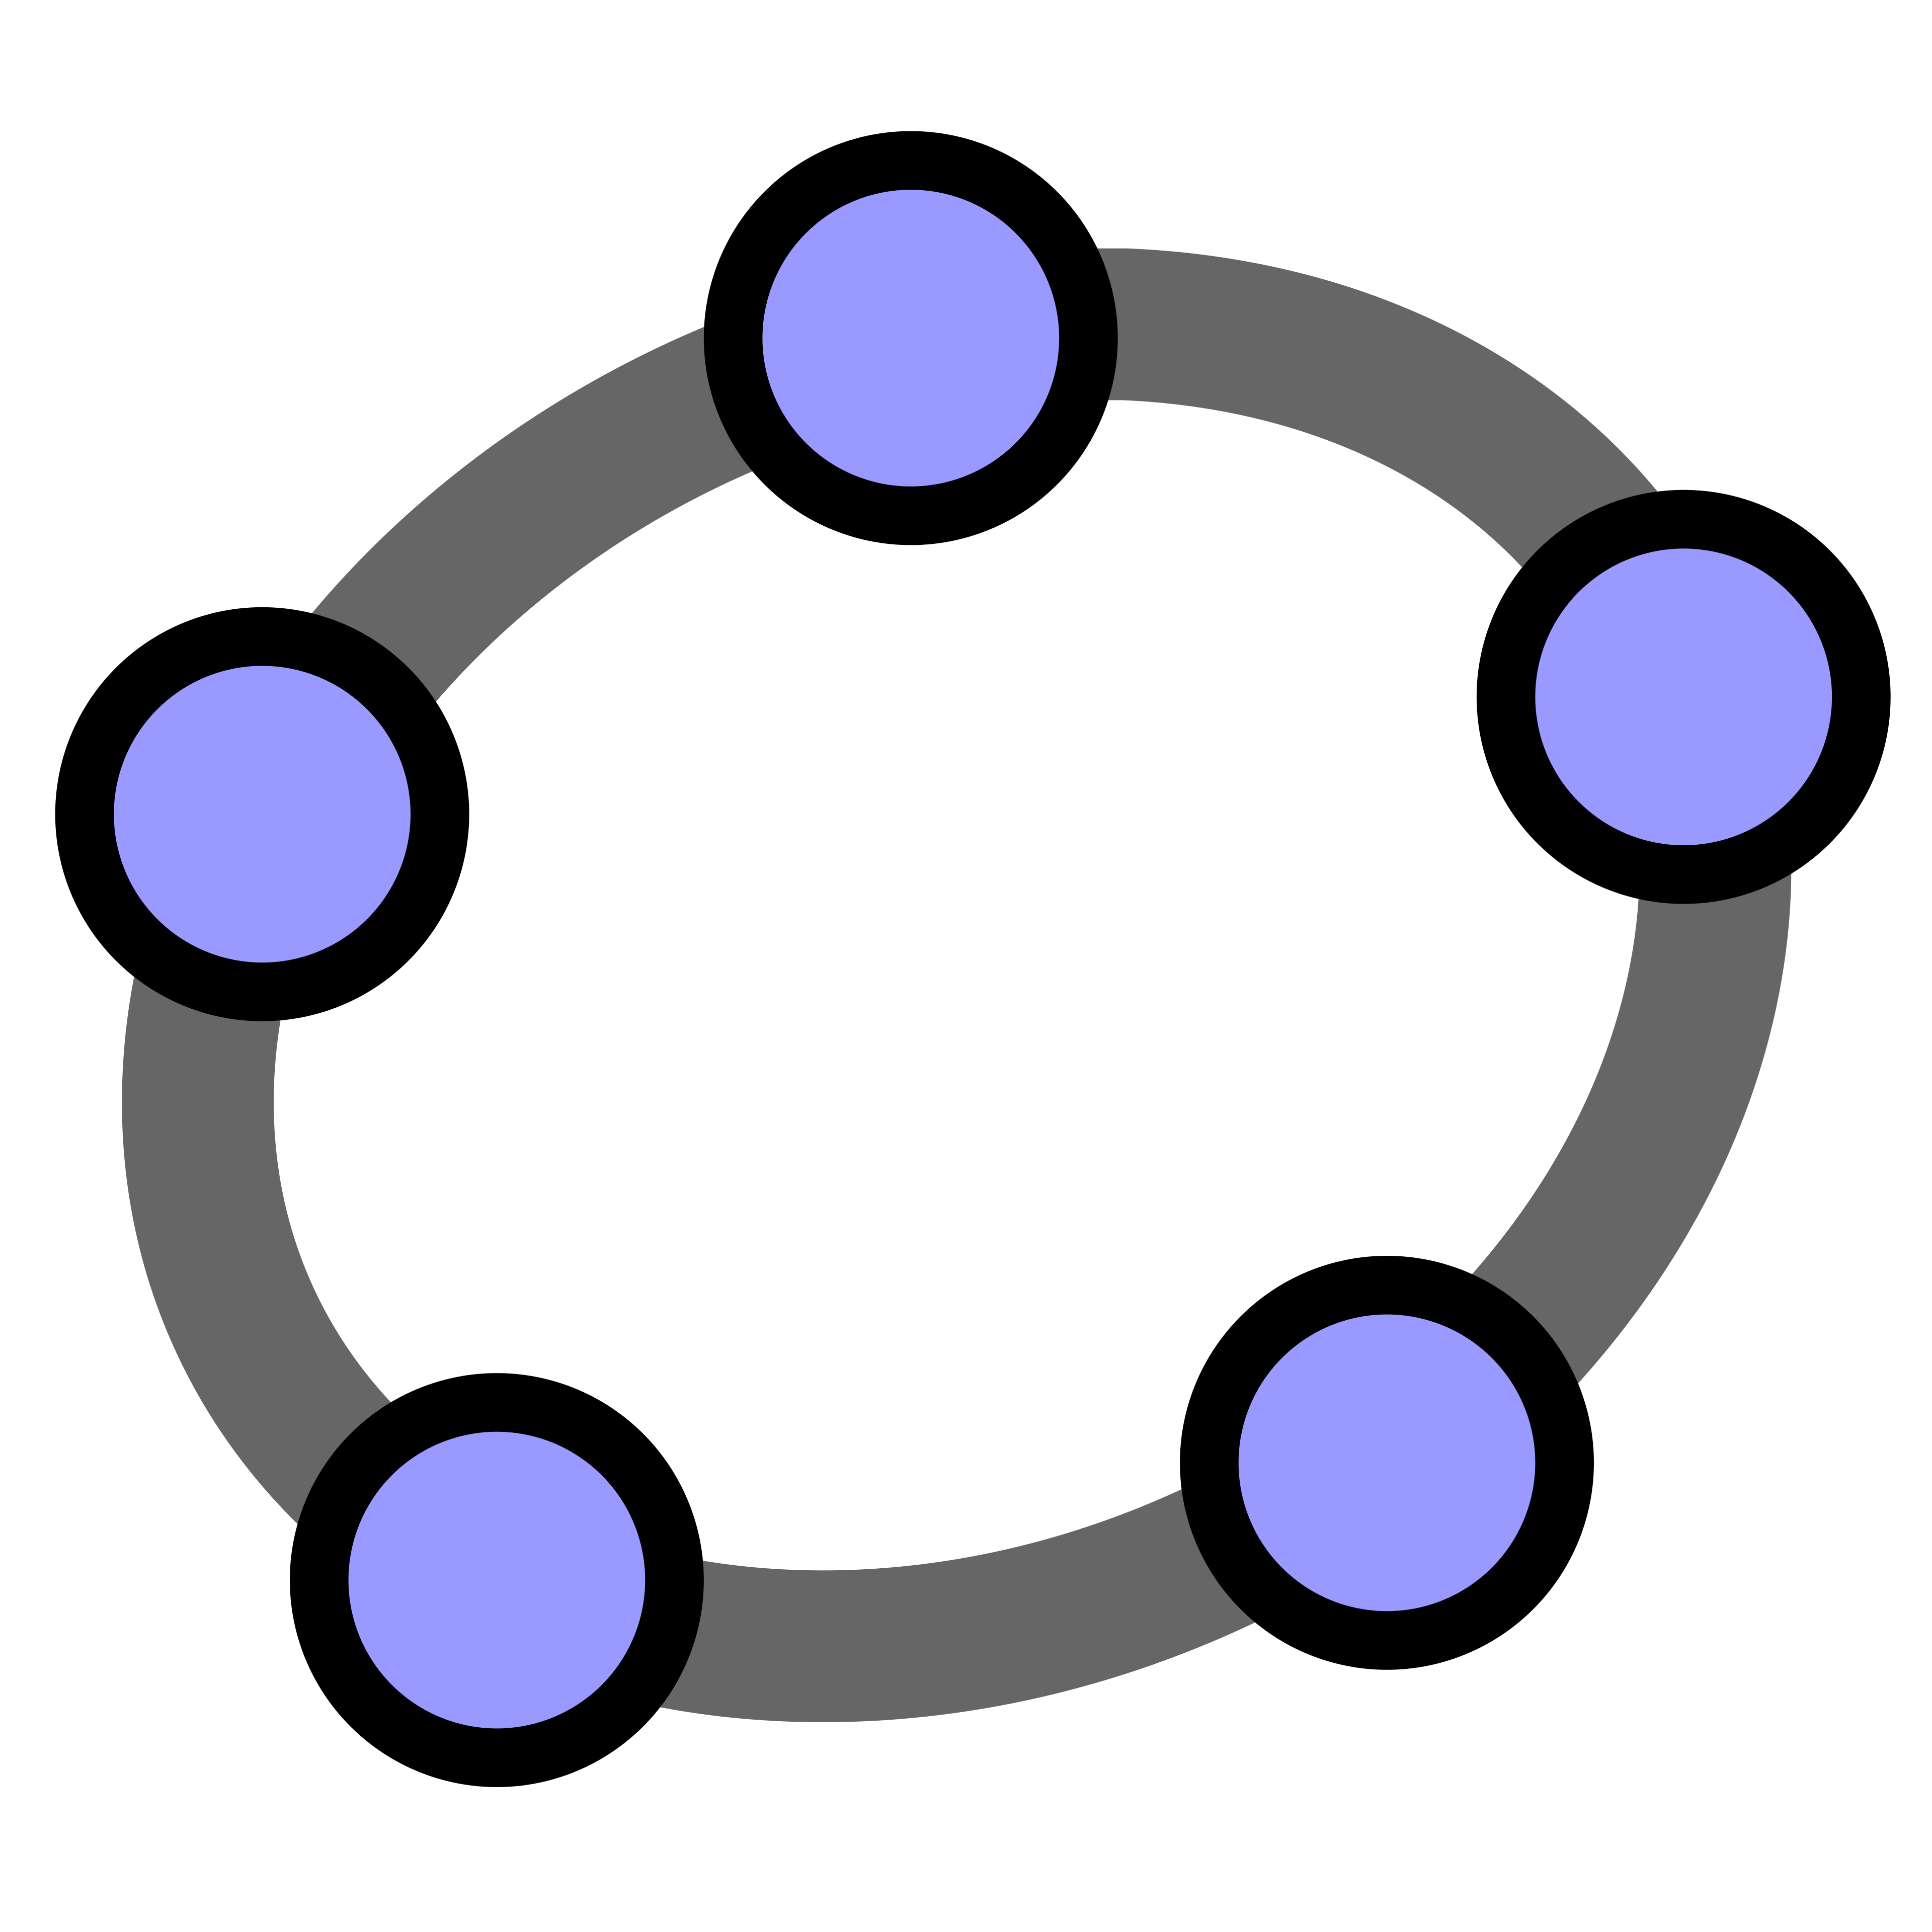
\includegraphics[width=3cm]{images/tools/geogebra.png}\end{center} \\ \hline
\textbf{Descripción:} Software matemático dinámico que permite representar gráficamente funciones, realizar construcciones geométricas y analizar fenómenos algebraicos y de cálculo. \\ \hline
\textbf{Uso:} Visualización de gráficas para la simulación \\ \hline
\textbf{Recurso en línea:} \href{https://www.geogebra.org/?lang=es}{\textit{Pulsa aquí}} \\
\hline
\end{tabular}
\vspace{10pt}
\caption{Tabla: Herramienta GeoGebra}
\end{table}

\vspace{-20pt}